During training, the network was evaluated on multiple metrics: the \gls{iou}\footnote{In this section, the term \gls{iou} will be used to describe all types of \gls{iou} losses}, the F1-Score and the \gls{map}. For each training, the weights with the best \gls{map} were kept.  

\section{Performance statistics}
\subsection{Model modifications}
Off all the modifications made on the network, by it on the architecture itself or with the training procedure, the most performance boost over a "vanilla" or unmodified YOLOv4 was the use of the CV2 library during training, which allowed the use of the Mosaic data augmentation. Increasing the input size also gave way to improvements in the accuracy for class prediction, but with a lower \gls{iou}. It should be noted that using CV2 during training has a significant negative impact on training time lasting up to $25\%$ longer\footnote{from $\sim 25$ hours to more than $\sim 30$ hours}. 

The best performing model uses CV2 augmentations during training, along with the \gls{giou} loss and the \gls{dnms}. This model is trained on the last version of the dataset, which uses $500 \times 500$ pixels images with reuses of objects. The CV2 augmentations gives the model a better robustness against occlusion, a recurring issue in the dataset. The larger input size give a better class accuracy. The dataset used was the V4, or the $1000 \times 1000$ pixels images, with random coordinates.  


\begin{table}[h]
	\centering
	\begin{tabular}{@{}llll@{}}
		\toprule
			      & Kilns           & Barrows         & Celtic Field    \\ \midrule
			      Faster R-CNN\\ (Verschoof-van der Vaart 2019) \cite{wouter2019}& ---             & 55\%             & 58\%             \\
			      Faster R-CNN\\ (Verschoof-van der Vaart 2020) \cite{wouter2020}& 12\% & 73\%             & 66\%             \\
			      Vanilla YOLOv4                & 63.04\%          & 77.04\%          & 85.73\%          \\
			      YOLOv4 + CV2 + GIOU + DNMS    & \textbf{82.37\%} & \textbf{80.50\%} & \textbf{95.92\%} \\ \bottomrule
	\end{tabular}
			      \caption{Per class precision of 3 chosen models. The best performing YOLO significantly outperforms the vanilla model and the Faster-RCNN. Precision values for Faster RCNN were chosen using the best performing model based on the maF1 Score.}
			      \label{tab:resClasses}
\end{table}

Table~\ref{tab:resClasses} shows the results of training for a vanilla YOLOv4, i.e. a non modified architecture \textit{versus} the best performing model with \gls{giou} and Distance \gls{nms}. CV2 data augmentations were also used.

\begin{table}[h]
	\centering
	\begin{tabular}{@{}lllllll@{}}
		\toprule
			      & Precision     & Recall        & F1-Score      & Av. IOU    & map@50         & MCC \\ \midrule
			      Faster R-CNN\\ (Verschoof-van der Vaart 2019)\cite{wouter2019} & ---           & ---           & 0.63          & ---            & ---            &     \\
			      Faster R-CNN\\ (Verschoof-van der Vaart 2020)\cite{wouter2020} & ---           & ---           & 0.37 & ---            & ---            &     \\
			      Vanilla YOLOv4                & 0.58          & 0.84          & 0.69          & 45.75          & 75.27          &   0.297  \\
			      YOLOv4 + CV2 + GIOU + DNMS    & \textbf{0.64} & \textbf{0.93} & \textbf{0.76} & \textbf{57.48\%} & \textbf{86.27\%} &     \textbf{0.305} \\ \bottomrule
	\end{tabular}
			      \caption{General Statistic based on all classes. Again, the best model significantly outperforms the vanilla model.}
			      \label{tab:resultsGen}
\end{table}

Table~\ref{tab:resultsGen} shows statistics for all classes. F1-Score for the \gls{yolo} models are good. The best model obtains a very high map@50 at over 86\% and a good average IOU nearing 60\%.

\begin{table}[h]
	\centering
	\begin{tabular}{@{}llllll@{}}
		\toprule
		                                                                                             & Precision     & Recall        & F1-Score      & Average IOU    & map@50         \\ \midrule
													     \begin{tabular}[c]{@{}l@{}}Vanilla YOLOv4\\ (not anchors optimised)\end{tabular}             & 0.58          & 0.84          & 0.69          & 45.75          & 75.27          \\
														     \begin{tabular}[c]{@{}l@{}}YOLOv4 + CV2 + GIOU + DNMS \\ (not anchor optimised)\end{tabular} & \textbf{0.64} & \textbf{0.93} & \textbf{0.76} & \textbf{57.48} & \textbf{86.27} \\ \midrule
															     \begin{tabular}[c]{@{}l@{}}Vanilla YOLOv4\\ (anchors optimised)\end{tabular}                 & 0.58          & 0.84          & 0.69          & 45.75          & 75.27          \\
																     \begin{tabular}[c]{@{}l@{}}YOLOv4 + CV2 + GIOU + DNMS\\ (anchor optimised)\end{tabular}      & \textbf{0.64} & 0.91          & \textbf{0.76} & \textbf{58.13} & 85.72          \\ \bottomrule
	\end{tabular}
	\caption{General Statistic based on all classes, with base anchors \textit{versus} optimised anchors . Interestingly, the optimised anchors model slightly outperforms the base anchors model with the average IOU, but only by less than a percent, while being inferior or similar in other metrics.}
	\label{tab:resGenAnchors}
\end{table}


Another question that needed to be answered was the impact of the anchors on the performance of the models. Here, 4 models were trained on the version 4 of the dataset: a simple "vanilla" \gls{yolo} model with and without optimised anchors and the best performing model with and without optimised anchors. Table~\ref{tab:resGenAnchors}. Here, we can see that while the average \gls{iou} is slightly improved by the optimised anchors, other metrics are similar or inferior to the model without optimised anchors. 

\begin{figure}[h!]
	\centering
	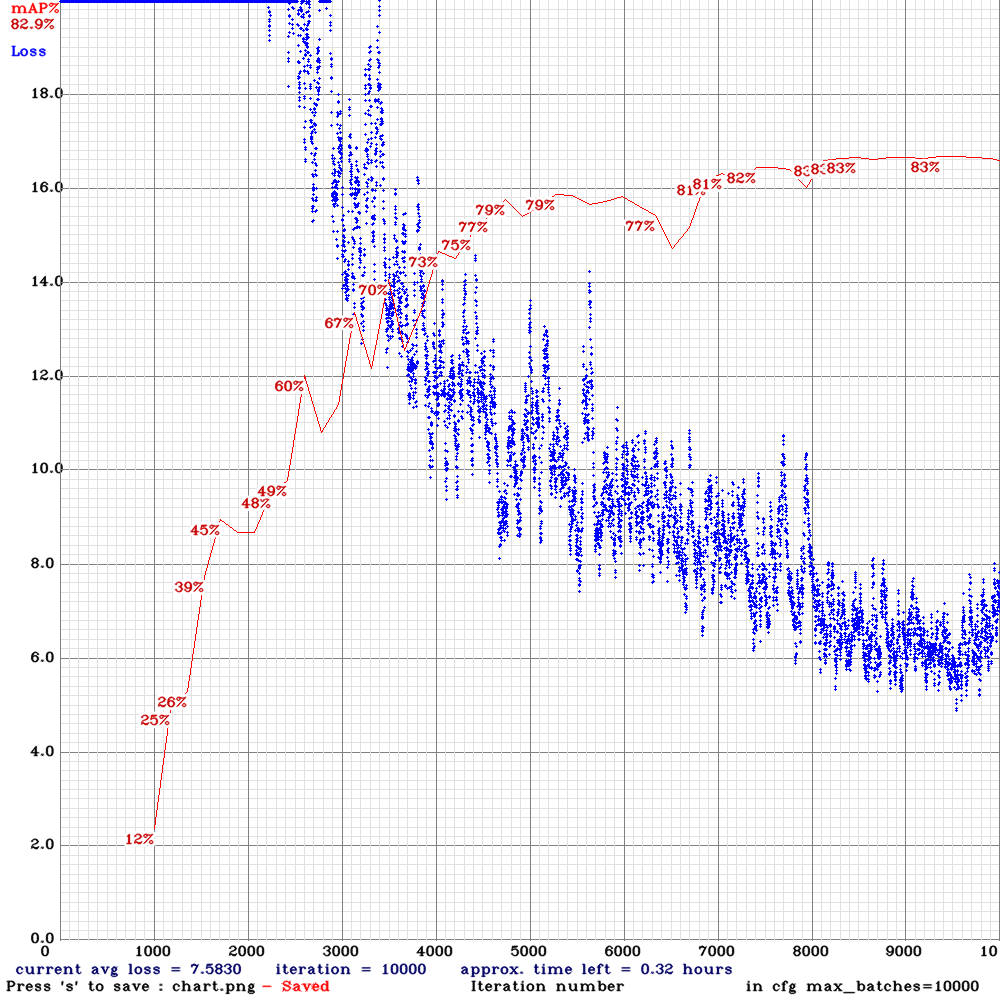
\includegraphics[width=0.5\textwidth]{chart_yolov4-custom-CV2}
	\caption[]{Evolution of loss and map@50 during training epochs of the best performing model}
	\label{fig:lossYOLO}
\end{figure}

Figure~\ref{fig:lossYOLO} shows the loss and \gls{map} of the best performing model throughout loss. The loss converge to a stable value, while \gls{map} rises. It also seems that the dreaded overfitting do not seems to happen, as the value of map does not diminishes at the end of training. 


\begin{table}[H]
	\centering
	\begin{tabular}{ll|ccc}
		&              & \multicolumn{1}{l}{} & \multicolumn{1}{l}{Predictions} & \multicolumn{1}{l}{} \\ \cline{3-5} 
								      &              & Kiln                 & Celtic Field                    & Barrow               \\ \hline
								      \multicolumn{1}{l|}{}      & Kiln         & 0.93           & 0.01                      & 0.05           \\
								      \multicolumn{1}{l|}{Truth} & Celtic Field & 0.01 & 0.95    & 0.06 \\
								      \multicolumn{1}{l|}{}      & Barrow       & 0.02 & 0.19 & 0.73
	\end{tabular}
	\caption{Confusion Matrix of the best performing model.}
	\label{tab:confMatYOLO}
\end{table}

A confusion matrix has been computed for the best performing model, and is reproduced in Table\ref{tab:confMatYOLO}, which indicates us which class are confused. Interestingly, while most classes are predicted accurately, the most confusion between classes happen between barrows and Celtic fields.  

\subsection{Impact of anchors on performance}
While training, I also wanted to see the impact that a modifications of the anchors of the network had on performance. Computing anchors tailored for the dataset can be done the following command:

\begin{verbatim}
./darknet detector calc_anchors data/obj.data -num_of_clusters 9\\
-width <width> -height <height> 
\end{verbatim}

With \verb|<width>| and \verb|<height>| being the width and height of the images. 

Replacing the anchors in the configuration file is done by modifying 3 lines in the YOLO modules called \verb|anchors|. 

While class prediction performance is not vastly affected by a change in anchors, the average \gls{iou} is. This make senses, as the anchors are used by the model to correctly place bounding boxes. Bad anchors will produce bad bounding boxes, which will in turn reduce the \gls{iou} of the prediction \textit{versus} the ground truth.


\section{Detection on sample images}
Thanks to darknet, it is fairly easy to use the model to perform inference on one or multiple images. To infer on a single TIF image, one must first create tiles or segments of the image. If not done, darknet would simply downsample the image to a fixed size, losing massive amounts of details. The user can use the script \verb|cutDataset.py|, which will segment every image in the dataset into $1000 \times 1000$ tiles. Inference is then done on those tiles, and results are saved in a text file.

\section{Integration into a GIS}
The end result of this project was to create a detection model that worked on \gls{lidar} surveys e.g. images. However, analysis of those results isn't done on the raw images, but on \gls{gis}, such as QGIS\cite{QGIS_software}. Developing some way to integrate the detection results into this kind of software was a priority. Thankfully, QGIS allows for the import of \gls{csv} database as shape files. This meant that the detection results could simply be integrated into a database, where each line contained the position of the bounding box in the \gls{wkt} format along with the confidence and the class. 

\begin{figure}
	\centering
	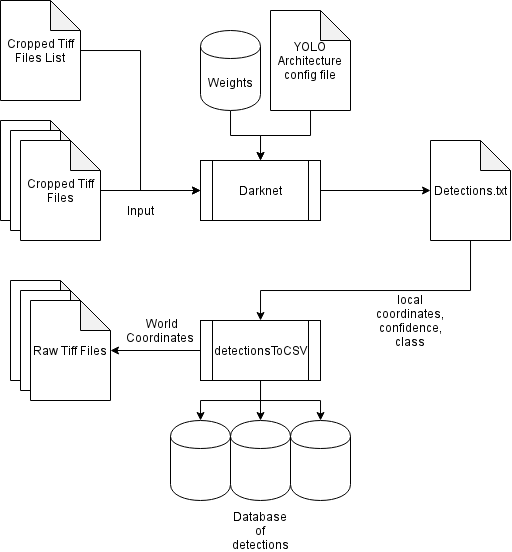
\includegraphics[width=0.8\textwidth]{dependenciesFull.png}
	\caption[Functional graph of the detection program]{Functional graph of the detection program. First the full size TIF are cropped into reasonable size images, and a list of those images is also generated. Then the darknet detector uses the trained weights and the configuration file to perform inference on those images. The detection results are stored in a text file. This text file is then read to extract the detection attributes, transform their coordinates from local to world and write the results to CSV databases.}
	\label{}
\end{figure}

This operation is done in a few steps. First the user crops the raw \gls{lidar} images into $1000 \times 1000$ chunks. This prevents the catastrophic loss of details that would happen with a downscale. Then inference is done on those images. \textbf{A "side effect" of using YOLO is the inference speed: on a few benchmark test, the model was able to infer on the entire dataset, i.e. about 3500 tiles or $\sim 500 km^2$ in about 8 minutes. } The detection results, with a confidence percentage, class and location of the bounding box of the detection are saved in a text file. 

The \verb|detectionsToCSV| script allows the user to take those detections results and create 3 databases of objects, one for each class. The scripts works by first finding the main image in which the cropped image was taken from. Then it uses the \verb|gdalinfo| command line utility to get the coordinates of the main image, and from that compute the coordinates of the bounding box in the world, which are then formatted into \gls{wkt} and written into the corresponding database. Some post-processing is done on the results: \textbf{YOLO seems to sometimes outputs very erroneous detections, in particular for Celtic Fields. Those detections have high confidence scores but are with a very low width and a high height}. A simple fix is to discard boxes where the ratio between width and height is over a threshold. 

As we cannot dare to write about object detection without showing examples of such detections, we shall show a few examples of successful detections on the base TIF images. 

\begin{figure}
	\centering
	\begin{subfigure}[b]{\textwidth}
		\centering
		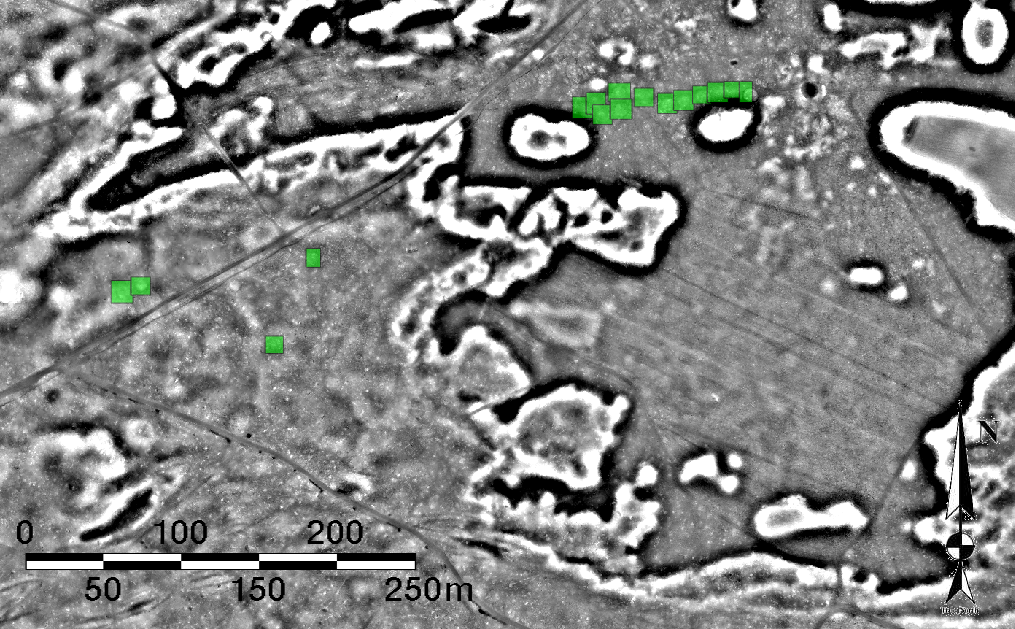
\includegraphics[width=\textwidth]{detectionsExample1}
		\caption[]{Detected charcoal kilns}    
		\label{fig:detectExample1}
	\end{subfigure}
	\begin{subfigure}[b]{\textwidth}  
		\centering 
		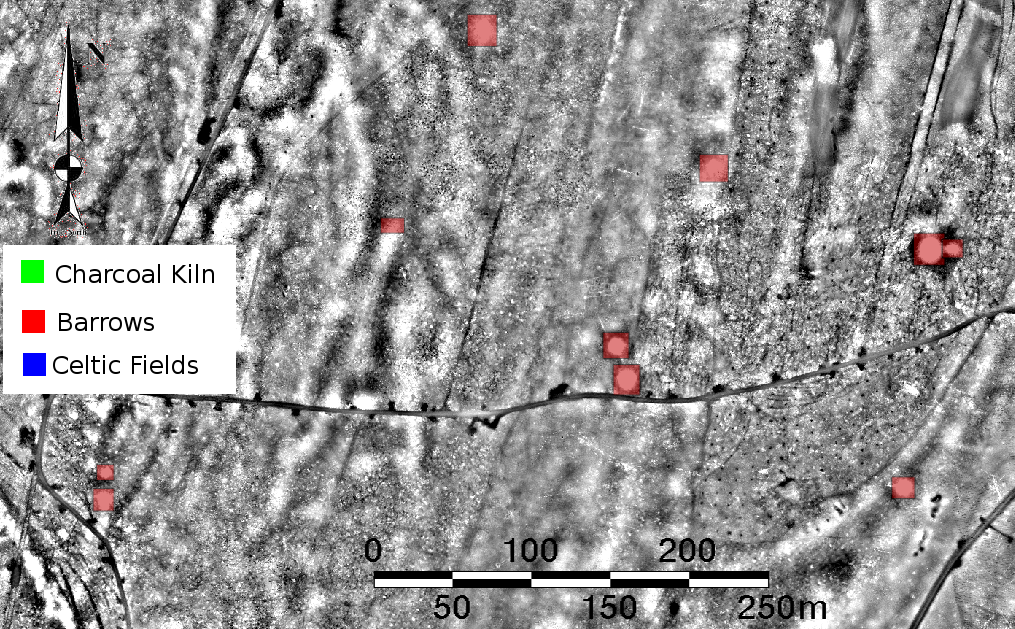
\includegraphics[width=\textwidth]{detectionsExample2}
		\caption[]{Detected barrows along a road in the Veluwe Region, Netherlands.}    
		\label{fig:detectExample2}
	\end{subfigure}
	\caption{Example of successful detections on visualized \gls{lidar} data. The red squares represents detected barrows, green are detected charcoal kilns and blue are detected Celtic fields. Screencaptures from QGIS}
\end{figure}


\begin{figure}[ht]
	\begin{subfigure}{\textwidth}
		\centering
		% include first image
		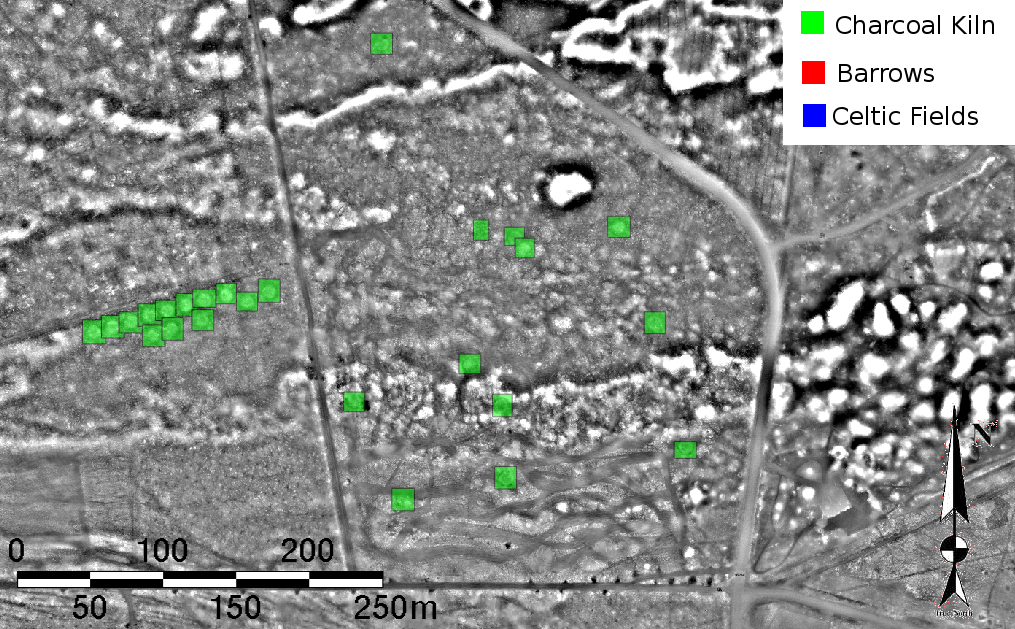
\includegraphics[width=\linewidth]{detectionsExample3}  
		\caption{Rows of charcoal kilns in the Veluwe Park.}
		\label{fig:detectionsExample3}
	\end{subfigure}
	\begin{subfigure}{\textwidth}
		\centering
		% include second image
		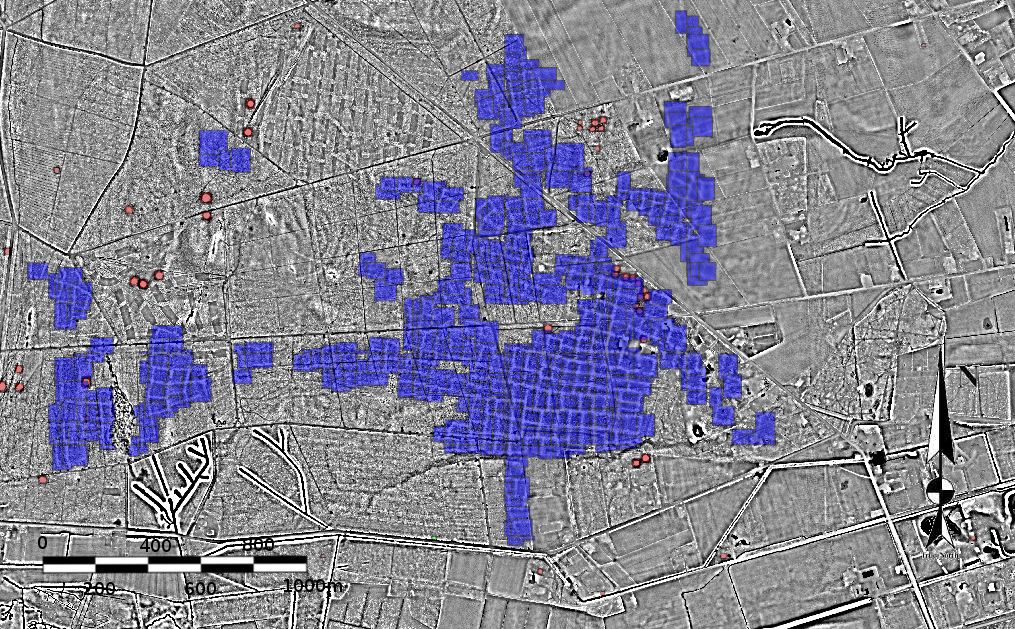
\includegraphics[width=\linewidth]{detectionsExample4}  
		\caption{Celtic fields and barrows in a large region of the Veluwe Park, Netherlands.}
		\label{fig:}
	\end{subfigure}
	\caption{Examples of successful detections of the 3 classes of objects. }
	\label{fig:}
\end{figure}
